\documentclass[10pt]{article}

\usepackage[latin1]{inputenc}
\usepackage{amsmath, amssymb, amsfonts, amsthm} \usepackage{upgreek} \usepackage{amsthm} \usepackage{fullpage}
\usepackage{graphicx}
\usepackage{cancel}
\usepackage{subfigure}
\usepackage{mathrsfs}
\usepackage{outlines}
\usepackage[font={sf,it}, labelfont={sf,bf}, labelsep=space, belowskip=5pt]{caption}
\usepackage{hyperref}
% \usepackage{minted}
\usepackage{titling}
\usepackage{xifthen}
\usepackage{color}

\usepackage{fancyhdr}
\usepackage[title]{appendix}
\usepackage{float}

\usepackage{siunitx}

\newcommand{\TODO}[1]{\textbf{****** {\bf{[#1]}} ******}}

\usepackage{prettyref}
\newrefformat{sec}{Section~\ref{#1}}
\newrefformat{tbl}{Table~\ref{#1}}
\newrefformat{fig}{Figure~\ref{#1}}
\newrefformat{chp}{Chapter~\ref{#1}}
\newrefformat{eqn}{\eqref{#1}}
\newrefformat{set}{\eqref{#1}}
\newrefformat{alg}{Algorithm~\ref{#1}}
\newrefformat{apx}{Appendix~\ref{#1}}
\newrefformat{prop}{Proposition~\ref{#1}}
\newcommand\pr[1]{\prettyref{#1}}

\usepackage{mathtools}

\DeclareMathOperator{\tr}{tr}
\DeclareMathOperator{\sgn}{sgn}
\DeclareMathOperator{\sinc}{sinc}
\DeclareMathOperator{\rref}{rref}
\DeclareMathOperator{\cof}{cof}
\DeclareMathOperator*{\sym}{sym}
\DeclareMathOperator{\image}{im} % image space of a linear transform

\DeclareMathOperator{\diag}{diag}
\DeclareMathOperator*{\argmax}{argmax}
\DeclareMathOperator*{\argmin}{argmin}
\newcommand{\defeq}{\vcentcolon=}

\renewcommand{\Re}{\operatorname{Re}} \renewcommand{\Im}{\operatorname{Im}}

\providecommand{\norm}[1]{\lVert#1\rVert}
\providecommand{\normlr}[1]{\left\lVert#1\right\rVert}

\providecommand{\tpder}[4]{\frac{\partial^3 #1}{\partial #2 \partial #3 \partial #4}}

\def\jointset{\mathcal{J}}
\def\actjoints{\mathcal{J}'}
\def\rodset{\mathcal{R}}

\renewcommand{\vec}[1]{{\bf #1}}
\def\xflat{\vec{x}^*_\text{2D}}
\def\xdeploy{\vec{x}^*_\text{3D}}
\def\xtgt{\vec{x}_\text{tgt}}

\usepackage{bm}
\def\torques{{\bm \tau}}

\def\R{\mathbb{R}}

\def\normal{{\bm n}}
\def\n{\normal}
\def\a{\vec{a}}
\def\b{\vec{b}}
\def\c{\vec{c}}
\def\d{\vec{d}}
\def\t{\vec{t}}
\def\x{\vec{x}}
\def\X{\vec{X}}
\def\y{\vec{y}}
\def\z{\vec{z}}
\def\u{\vec{u}}
\def\f{\vec{f}}
\def\g{\vec{g}}
% \def\w{\boldsymbol{\omega}}
\def\w{\vec{w}}
\def\wn{\norm{\w}}
\def\p{\vec{p}}
\def\q{\vec{q}}
\def\v{\vec{v}}
\def\e{\vec{e}}
\def\ue{\vec{u}^\e}
\def\fu{\pder{\f}{u}}
\def\fv{\pder{\f}{v}}
\def\strain{\varepsilon}
\def\stress{\sigma}
\def\kb{\kappa \b}
\def\kbi{(\kappa \b)_i}
\def\kn{\bm{\kappa}}
\def\k{\kappa}
\def\R{\, \mathbb{R}}
\def\L{\, \mathcal{L}}
\def\deployAmount{\overline{\alpha}}
\def\deployTgt{\overline{\alpha}^\text{tgt}}

\def\wref{\hat{\w}}

\providecommand{\abs}[1]{\lvert#1\rvert}
\providecommand{\norm}[1]{\lVert#1\rVert}
\providecommand{\normlr}[1]{\left\lVert#1\right\rVert}
\providecommand{\dx}{\, \mathrm{d}x}
\providecommand{\ds}{\, \mathrm{d}s}
\providecommand{\lint}[3]{\int_{#1}^{#2} \! #3 \, \ds}
% \providecommand{\vint}[2]{\int_{#1} \! #2 \, \mathrm{d}x}
% \providecommand{\sint}[2]{\int_{\partial #1} \! #2 \, \mathrm{d}A}
\renewcommand{\div}{\nabla \cdot}
\providecommand{\cross}{\times}
\providecommand{\curl}{\nabla \cross}
\providecommand{\grad}{\nabla}
\providecommand{\laplacian}{\bigtriangleup}
\providecommand{\shape}{\Omega}
\providecommand{\mesh}{\mathcal{M}}
\providecommand{\boundary}{\partial \shape}
\providecommand{\vint}[3][\x]{\int_{#2} \! #3 \, \mathrm{d}#1}
\providecommand{\sint}[3][\x]{\int_{#2} \! #3 \, \mathrm{d}A(#1)}
\providecommand{\pder}[2]{\frac{\partial #1}{\partial #2}}
\providecommand{\spder}[3]{\frac{\partial^2 #1}{\partial #2 \partial #3}}
\providecommand{\spderx}[1]{\frac{\partial^2 #1}{\partial \x^2 }}
\providecommand{\tder}[2]{\frac{\mathrm{d} #1}{\mathrm{d} #2}}
\providecommand{\evalat}[2]{\left.#1\right|_{#2}}
\renewcommand{\vec}[1]{{\bf #1}}

\providecommand{\shapeder}[2]{{\mathrm{d} #1}[#2]}
\providecommand{\matder}[1]{\dot{#1}}

\providecommand{\tderatzero}[2]{\left.\frac{\mathrm{d} #1}{\mathrm{d} #2}\right|_{#2 = 0}}

\providecommand{\compose}{\circ}
\providecommand{\surface}{\Gamma}
\providecommand{\surfacegrad}{\nabla_\surface}
\providecommand{\surfacediv}{\surfacegrad \cdot}
\providecommand{\surfacelaplacian}{\laplacian_\surface}

\providecommand{\epssurface}{{\Gamma_\epsilon}}
\providecommand{\epssurfacegrad}{\nabla_\epssurface}
\providecommand{\epssurfacediv}{\epssurfacegrad \cdot}
\providecommand{\epsnormal}{\normal_\epsilon}
\providecommand{\epsnormalmat}{\tilde{\normal}_\epsilon}
\providecommand{\epsphi}{\phi_\epsilon}
\providecommand{\normalmatder}{\dot{\normal}}
\providecommand{\shapefunc}{{\bm \phi}}

\def\vt{\vec{v}_t}
\def\k{\kappa}

\providecommand\ts[1]{\widehat{\vec{t}^{#1}}}
\providecommand\ds[2]{\widehat{\vec{d}^{#1}_{#2}}}
\providecommand\rd[2]{\underline{\vec{d}^{#1}_{#2}}}
\providecommand\rds[2]{\widehat{\underline{\vec{d}^{#1}_{#2}}}}
\providecommand{\PXport}[1]{P_{\ts{#1}}^{\t^{#1}}}
\providecommand{\ki}[2]{(\k_{#1})_i^{#2}}

\newtheorem{lemma}{Lemma}
\newtheorem{proposition}{Proposition}
\newtheorem{corollary}{Corollary}

\usepackage{mathtools}
\newcases{mycases}{\quad}{%
  \hfil$\m@th\displaystyle{##}$}{$\m@th\displaystyle{##}$\hfil}{\lbrace}{.}
\makeatother


\newcommand{\documenttitle}{Quantifying Single DoF Behavior of X-Shells}

% \allowdisplaybreaks
\pagestyle{fancy}
\headheight 24pt
\headsep    12pt
\lhead{\documenttitle}
\rhead{\today}
\fancyfoot[C]{} % hide the default page number at the bottom
\lfoot{}
\rfoot{\thepage}
\renewcommand{\headrulewidth}{0.4pt}
\renewcommand\footrulewidth{0.4pt}

\def\mpa{\si{\mega\pascal} }
\def\mm{\si{\milli\meter} }

\newcommand*{\rom}[1]{\expandafter\@slowromancap\romannumeral #1@}
\newcommand{\RN}[1]{\textup{\uppercase\expandafter{\romannumeral#1}}}

\makeatletter

\setlength{\droptitle}{-50pt}
\title{\documenttitle}
\author{Julian Panetta}

% BEGIN DOCUMENT
\begin{document}
\maketitle

One of the defining characteristics of X-Shells is that they behave almost like
single DoF linkages: they possess a single easily actuated deployment path.
This document derives a method to measure the extent to which this property holds
for a given design.

\section{Deformation Energy Gaps by Spectral Analysis}
The first approach one might try is to analyze the spectrum of the elastic
energy Hessian at sampled points along the deployment path. At a configuration
along this path, one might expect the eigenmode corresponding to the smallest
eigenvalue to indicate the (infinitesimal) deformation moving along the
deployment path, since it is the lowest energy deformation that can be applied
to the structure. Then we would hope for a large gap between this smallest
eigenvalue and the next smallest, indicating that any other deformation mode is
much more difficult to apply. However, upon analyzing the Hessian spectra of
some of our X-Shell designs, we find that even designs whose physical
prototypes behaved well---like the Barcelona Pavilion---can have very
little separation between their smallest eigenvalues, or possibly even have a
lowest energy mode involving out-of-plane bending instead of expansion
(\texttt{AsymmetricWingsPointy}). In these cases, though, the undesirable low
energy modes were not problematic because they were not actually excited by actuation
forces; a single deployment path was still singled out well.

\section{Deployment Stiffness Gaps by Constrained Optimization}
Another way to quantify the uniqueness of the deployment path is to measure
the gap in energy required to deploy the structure by a particular increment
(a) along the most efficient direction and (b) along the second most efficient
orthogonal direction. If this gap is large, we can be confident that the
deployment path will be robust to changes in the distribution of actuation
forces.

For this analysis, we need some measure of the amount the structure has deployed.
In our X-Shells paper, we use the average joint opening angle,
but we could instead use, e.g., a measure of the structure's bounding box size or
surface area. For consistency with the paper, we denote the degree of deployment
by $\deployAmount(\x)$ and write its derivative as $\pder{\deployAmount}{\x}(\x) = \a^T$.
Then an optimal deployed configuration along the path can be found by solving:
$$
\x^*(\deployTgt) = \argmin_{\substack{\x \\ \deployAmount(\x) = \deployTgt}} E(\x).
$$
At this configuration, the following forces are enforcing the
deployment amount:
$$
\pder{E}{\x}(\x^*) = \lambda \a^T(\x^*).
$$
Now, we wish to measure the work needed to increase the deployment by some
small increment $\Delta \deployAmount$ in the first and second most efficient
ways. Around the current equilibrium, we consider a local quadratic
approximation to the energy increase and a linearized deployment measure and
look for the most efficient displacement step $\d_1$:
$$
\d_1 \defeq \argmin_{\a^T \d = \Delta \deployAmount} \pder{E}{\x} \d + \frac{1}{2} \d^T H \d,
$$
where $H = \spderx{E}$.
This optimal step can be found by solving the KKT system:
\begin{gather*}
\begin{bmatrix}
    H & \a \\
    \a^T & 0
\end{bmatrix}
\begin{bmatrix}
    \d_1 \\ \mu
\end{bmatrix}
=
\begin{bmatrix}
    -\pder{E}{\x}^T \\ \Delta \deployAmount
\end{bmatrix}
= 
\begin{bmatrix}
    -\lambda \a \\ \Delta \deployAmount
\end{bmatrix}
\\
\Longleftrightarrow \quad 
    \d_1 = -(\lambda + \mu)H^{-1} \a, \quad \a^T \d_1 = \Delta \deployAmount
\\
    -(\lambda + \mu)\a^T H^{-1} \a = \Delta \deployAmount, \quad
\boxed{
    \d_1 = \frac{\Delta \deployAmount}{\a^T H^{-1} \a} H^{-1} \a.
}
\end{gather*}
The corresponding energy increment is then:
$$
\Delta E_1 =
\pder{E}{\x} \d_1 + \frac{1}{2} \d_1^T H \d_1
= \lambda \a^T \d_1 + \frac{1}{2} \d_1^T H \d_1
= \lambda \Delta \deployAmount + \frac{1}{2 \a^T H^{-1} \a}(\Delta \deployAmount)^2
= \lambda \Delta \deployAmount + \frac{(\Delta \deployAmount)^2}{2} \frac{1}{\norm{\a}_{H^{-1}}^2}.
$$
Thus, we see the initial force needed to increment the deployment is proportional to $\lambda$
(a standard interpretation of the Lagrange multiplier), while the stiffness along the
deployment path is proportional to $\frac{1}{\norm{\a}_{H^{-1}}^2}$. Note, if $\a$
happens to be an eigenvector of $H$, this is simply the corresponding stiffness eigenvalue.

Now, let us consider the \emph{second} most efficient deployment step $\d_2$. We ask this step
to be $M-$orthogonal to $\d_1$, where $M$ is the X-Shell's mass matrix:
$$
\d_2 \defeq \argmin_{\substack{\a^T \d = \Delta \deployAmount \\ \d_1^T M \d = 0}}
        \lambda \a^T \d + \frac{1}{2} \d^T H \d.
$$
Introducing Lagrange multipliers $\mu$ and $\gamma$ for the two constraints, we have the KKT system for $\d_2$:
\begin{gather*}
\begin{bmatrix}
    H & \a & M \d_1 \\
    \a^T & 0 & 0 \\
    (M \d_1)^T & 0 & 0
\end{bmatrix}
\begin{bmatrix}
    \d_2 \\ \mu \\ \gamma
\end{bmatrix}
= 
\begin{bmatrix}
    -\lambda \a \\ \Delta \deployAmount \\ 0
\end{bmatrix}
\\
\Longleftrightarrow \quad 
    \d_2 = -H^{-1} \begin{bmatrix} \a & M \d_1 \end{bmatrix}
                   \begin{bmatrix}\lambda + \mu \\ \gamma\end{bmatrix}, \quad
    \a^T \d_2 = \Delta \deployAmount, \quad
    \d_1^T M \d_2 = 0.
\end{gather*}
The constraints give us a linear system to solve for the Lagrange multipliers:
\begin{align*}
\begin{bmatrix} \Delta \deployAmount \\ 0 \end{bmatrix}
    &=
-\begin{bmatrix} \a & M \d_1 \end{bmatrix}^T 
H^{-1} \begin{bmatrix} \a & M \d_1 \end{bmatrix}
       \begin{bmatrix}\lambda + \mu \\ \gamma\end{bmatrix}
\\
    &=
    -\begin{bmatrix} \a^T H^{-1} \a & \a^T H^{-1} M \d_1 \\
                     \d_1^T M H^{-1} \a & \d_1^T M H^{-1} M \d_1
    \end{bmatrix}
       \begin{bmatrix}\lambda + \mu \\ \gamma\end{bmatrix}
\end{align*}
So the second most efficient deployment step is:
$$
    \d_2 = H^{-1} \begin{bmatrix} \a & M \d_1 \end{bmatrix}
\begin{bmatrix} \a^T H^{-1} \a & \a^T H^{-1} M \d_1 \\
                     \d_1^T M H^{-1} \a & \d_1^T M H^{-1} M \d_1
\end{bmatrix}^{-1}
\begin{bmatrix} \Delta \deployAmount \\ 0 \end{bmatrix}.
$$
The quadratic term of the energy increment is $\frac{1}{2}\d_2^T H \d_2 = $
\begin{gather*}
    \frac{1}{2}
    \begin{bmatrix} \Delta \deployAmount \\ 0 \end{bmatrix}^T
    \cancel{
        \begin{bmatrix} \a^T H^{-1} \a & \a^T H^{-1} M \d_1 \\
                             \d_1^T M H^{-1} \a & \d_1^T M H^{-1} M \d_1
        \end{bmatrix}^{-1}
            \begin{bmatrix} \a & M \d_1 \end{bmatrix}^T
            H^{-1}
            \begin{bmatrix} \a & M \d_1 \end{bmatrix}
    }
    \begin{bmatrix} \a^T H^{-1} \a & \a^T H^{-1} M \d_1 \\
                         \d_1^T M H^{-1} \a & \d_1^T M H^{-1} M \d_1
    \end{bmatrix}^{-1}
    \begin{bmatrix} \Delta \deployAmount \\ 0 \end{bmatrix}
\\
= 
    \frac{1}{2}
    \begin{bmatrix} \Delta \deployAmount & 0 \end{bmatrix}
        \begin{bmatrix} \a^T H^{-1} \a & \a^T H^{-1} M \d_1 \\
                             \d_1^T M H^{-1} \a & \d_1^T M H^{-1} M \d_1
        \end{bmatrix}^{-1}
    \begin{bmatrix} \Delta \deployAmount \\ 0 \end{bmatrix}
\\
= 
    \frac{(\Delta \deployAmount)^2}{2}
    \frac{\d_1^T M H^{-1} M \d_1}{\big(\a^T H^{-1} \a\big)\big(\d_1^T M H^{-1} M \d_1\big) - (\a^T H^{-1} M \d_1)^2}
= 
    \frac{(\Delta \deployAmount)^2}{2}
    \frac{1}{\norm{\a}_{H^{-1}}^2 - \left<\a, M \d_1\right>_{H^{-1}}^2 / \norm{M \d_1}_{H^{-1}}^2}
\end{gather*}
So the full energy increment for the second most efficient deployment step is:
$$
\Delta E_2 = \lambda \Delta \deployAmount + 
    \frac{(\Delta \deployAmount)^2}{2}
    \frac{1}{\norm{\a}_{H^{-1}}^2 - \left<\a, M \d_1\right>_{H^{-1}}^2 / \norm{M \d_1}_{H^{-1}}^2}.
$$
We note that the scale of $\d_2$ was chosen so that the linear term is guaranteed to be $\lambda \Delta \deployAmount$,
the same as the linear term of $\Delta E_1$.

We finally measure the relative gap in the deployment stiffness. This means we
ignore the linear term in the energy increment (which is the same for both
deployment paths by construction) and measure the relative change in the quadratic term:
$$
\frac{\Delta E_2 - \Delta E_1}{\Delta E_1 - \lambda \deployAmount} 
=
    \frac{1}{1 - \frac{\left<\a, M \d_1\right>_{H^{-1}}^2}{\norm{\a}_{H^{-1}}^2 \norm{M \d_1}_{H^{-1}}^2}} - 1,
$$
which we can interpret geometrically as 
$\frac{1}{1 - \cos(\theta)^2} - 1 = \csc(\theta)^2 - 1$ where $\theta$ is angle between $\a$ and $M \d_1$ according to the inverse Hessian metric.
Physically, this quantity tells us the (relative) difference in the \emph{additional} force needed to apply
a deployment increment along the best and second best deployment paths.

We note an interesting behavior when $M = I$ and $\a$ is a Hessian eigenvector:
then $\d_1$ and $\a$ are parallel, and the deployment energy gap becomes
infinite. This should be expected, however: if the optimal deployment
deformation is parallel to $\pder{\deployAmount}{\x}$, then it is impossible to
find an orthogonal direction that also changes the deployment amount to first order.

\section{Results}
For Etienne's original hyperboloid design, we see a substantial relative
stiffness gap of over 100 in both the planar and deployed configuration. This
indicates that the structure does truly behave like a single-DoF linkage.
Unfortunately, our other X-shell designs do not have quite as large a gap:

\begin{figure}[H]
    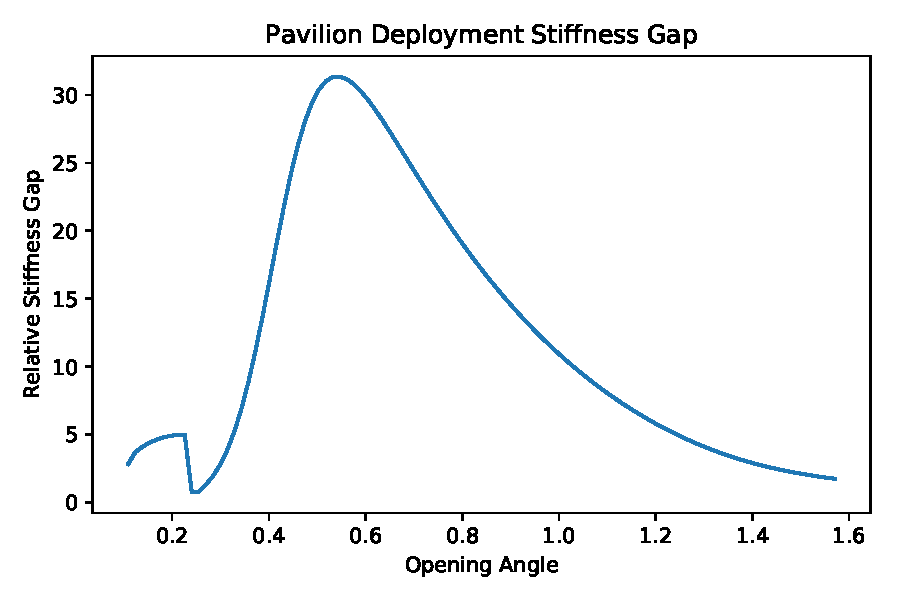
\includegraphics[width=0.33\textwidth]{plots/stiffness_gap_pavilion.pdf}
    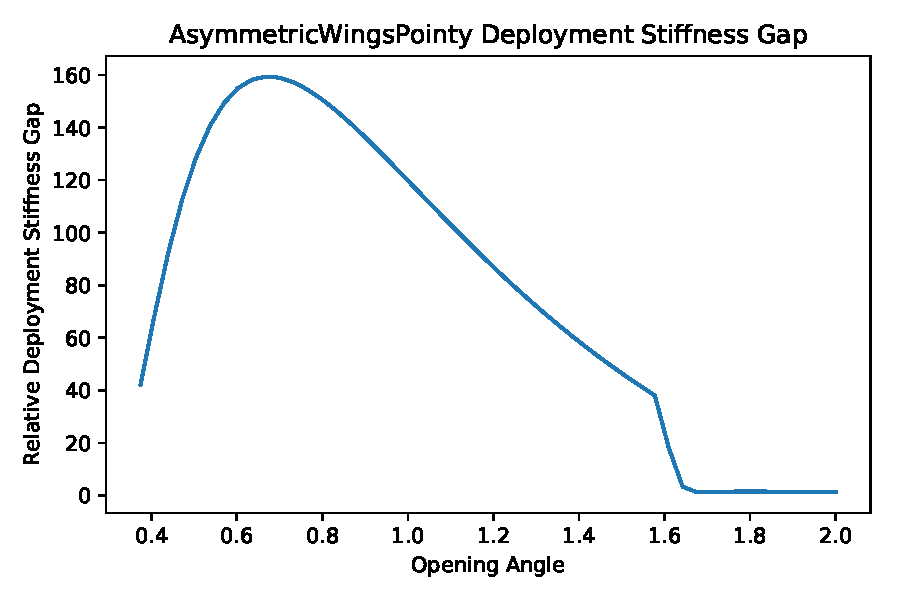
\includegraphics[width=0.33\textwidth]{plots/stiffness_gap_asymmetric_wings_pointy.pdf}
    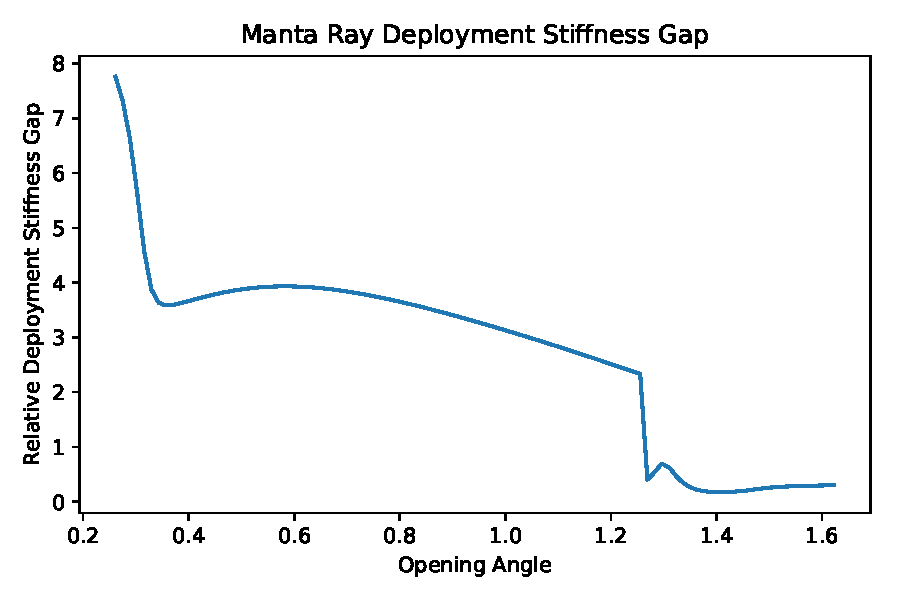
\includegraphics[width=0.33\textwidth]{plots/stiffness_gap_manta_ray.pdf}
\end{figure}

We note that there is often a dramatic drop in the stiffness gap at the moment
the structure buckles out of plane. In the case of the pavilion, the stiffness gap recovers
as the structure is further expanded (but then drops again as it nears its deployed shape).
The stiffness gaps of the three models in their final deployed states are
1.738, 1.259, and 0.301, respectively. So there is certainly a preferred deployment deformation, but
the amount of additional force required to branch off onto a different deployment path is not so
great in some designs.

However, the actual behavior may not be as bad as this analysis suggests: when we compare
the first- and second-most efficient deployment modes, sometimes they appear to produce visually
similar changes to the shape despite being $M$-orthogonal. Perhaps some better
measure of orthogonality could be used for defining the second deployment mode.

\section{Conclusion}
We propose a ``relative stiffness gap'' quantity to measure how tightly the
X-shell's design actually constrains it to follow the predicted deployment
path. This quantity is preferable to an analysis based on the Hessian
eigenvalues in that it ignores low energy modes that are unexcited by the
structure's deployment.

However, it is still valuable to inspect the lowest energy modes of the Hessian in
the deployed configuration to analyze how stiff the structure is and predict
likely deviations from the programmed shape due to external loads.

\end{document}
